\item ¿Cuál es la interfaz que ha recibido el mayor número de octetos?

\textbf{SO Centos}
Con ifInOctets vemos que interfaz tiene el mayor número de octetos en este caso es la 2, con ifDescr(2) vemos que la interfaz  2 es enpos3.
 
\ref{image:Pregunta4O}
\FloatBarrier
\begin{figure}[htbp!]
		\centering
		    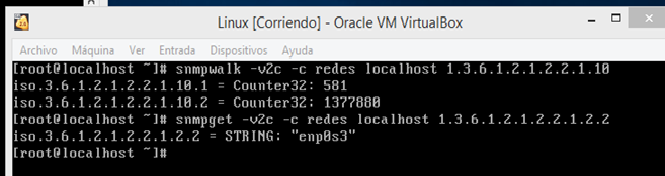
\includegraphics[width=.5 \textwidth]{../images/Pregunta4O.png} 
		\caption{El OID para ver los Octetos es 1.3.6.1.2.1.2.2.1.10}
		\label{image:Pregunta4O}
\end{figure}
\FloatBarrier

\textbf{SO Windows}
Con snmpwalk  podemos visualizar la tabla de las 26 interfaces con las que cuenta el so Windows y con la OID 1.3.6.1.2.1.2.2.1.10 (ifInOctets) se observan los octetos de cada una.

\ref{image:Pregunta4W}
\FloatBarrier
\begin{figure}[htbp!]
		\centering
		    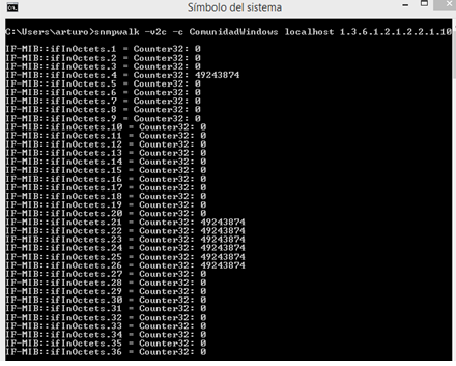
\includegraphics[width=.5 \textwidth]{../images/Pregunta4W.png} 
		\caption{tabla de las interfaces en Windows con sus Octetos}
		\label{image:Pregunta4W}
\end{figure}
\FloatBarrier

 Tenemos 7 interfaces que cuentan con la misma cantidad de octetos \textbf{(.4, .21, .22, .23, .24, .25, .26)} y podemos ver que esas interfaces son:
 
\ref{image:Pregunta4W2}
\FloatBarrier
\begin{figure}[htbp!]
		\centering
		    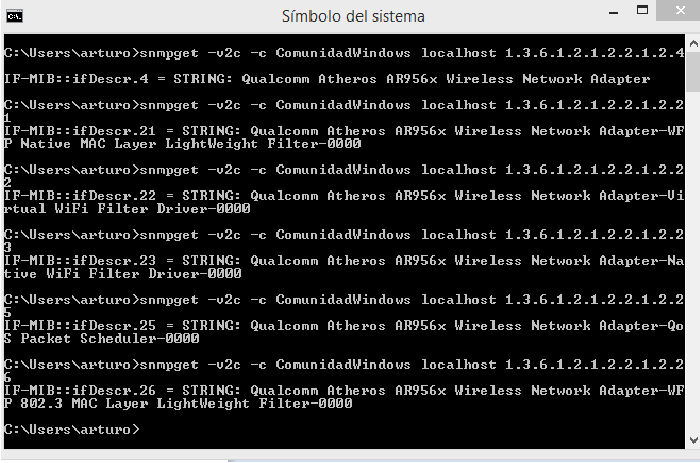
\includegraphics[width=.5 \textwidth]{../images/Pregunta4W2.png} 
		\caption{Interfaces}
		\label{image:Pregunta4W2}
\end{figure}
\FloatBarrier

\item Indica el número de octetos  de la interfaz que ha recibido el mayor número de octetos

\textbf{SO Centos}
enpos3 cuenta con 73986 octetos ifInOctets (OID 1.3.6.1.2.1.2.2.1.10.2) el cuál es \textbf{73986}.

\ref{image:Pregunta5C}
 \FloatBarrier
\begin{figure}[htbp!]
		\centering
		    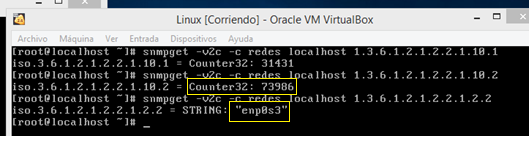
\includegraphics[width=.5 \textwidth]{../images/Pregunta5C.png} 
		\caption{Octetos en enp0s3}
		\label{image:Pregunta5C}
\end{figure}
\FloatBarrier

\textbf{SO Windows}
El número de octetos que han recibido las 7 interfaces por igual es \textbf{49243874}.

 \ref{image:Pregunta5W}
 \FloatBarrier
\begin{figure}[htbp!]
		\centering
		    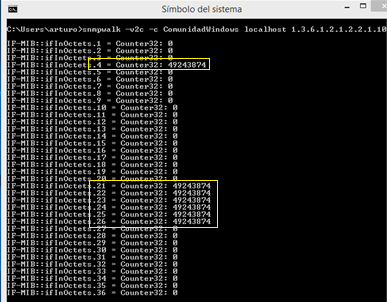
\includegraphics[width=.5 \textwidth]{../images/Pregunta5W.png} 
		\caption{Octetos en Windows}
		\label{image:Pregunta5W}
\end{figure}
\FloatBarrier

\item ¿Cuál es la MAC de esa interfaz?
\textbf{SO Centos}
Con ifphysAddres (OID 1.3.6.1.2.1.2.2.1.6.2 )podemos visualizar le Mac de enpos3 \textbf{8:0:27:91:60:40}.

 \ref{image:Pregunta6C}
 \FloatBarrier
\begin{figure}[htbp!]
		\centering
		    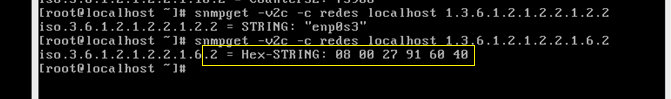
\includegraphics[width=.5 \textwidth]{../images/Pregunta6C.png} 
		\caption{Dirección Mac de Enp0s3}
		\label{image:Pregunta6C}
\end{figure}
\FloatBarrier

\textbf{SO Windows}
Con ifPhysAddress se puede observar que las 7 interfaces que tiene el número igualitario de octetos cuentan con la misma dirección Mac, para esto nos apoyamos del comando snmpwalk para poder visualizar en forma de lista las diferentes direcciones de cada interfaz con la que cuenta Windows. (OID 1.3.6.1.2.1.2.2.1.6)
Mac \textbf{18:4f:32:38:2a:3d}.

 \ref{image:Pregunta6W}
 \FloatBarrier
\begin{figure}[htbp!]
		\centering
		    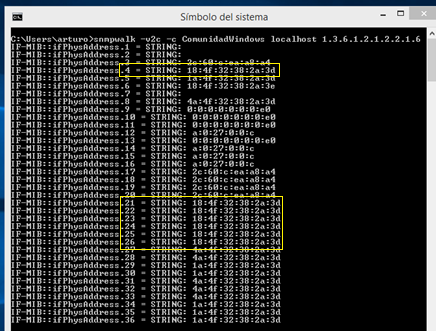
\includegraphics[width=.5 \textwidth]{../images/Pregunta6W.png} 
		\caption{Tabla de direcciones Mac en Windows}
		\label{image:Pregunta6W}
\end{figure}
\FloatBarrier